% -*- coding: utf-8 -*-
%!TEX program = xelatex
\ifx \allfiles \undefined
\documentclass[12pt]{ctexbook}
%\usepackage{xeCJK}
%\usepackage[14pt]{extsizes} %支持8,9,10,11,12,14,17,20pt

%===================文档页面设置====================
%---------------------印刷版尺寸--------------------
%\usepackage[a4paper,hmargin={2.3cm,1.7cm},vmargin=2.3cm,driver=xetex]{geometry}
%--------------------电子版------------------------
\usepackage[a4paper,margin=2cm,driver=xetex]{geometry}
%\usepackage[paperwidth=9.2cm, paperheight=12.4cm, width=9cm, height=12cm,top=0.2cm,
%            bottom=0.4cm,left=0.2cm,right=0.2cm,foot=0cm, nohead,nofoot,driver=xetex]{geometry}

%===================自定义颜色=====================
\usepackage{xcolor}
  \definecolor{mybackgroundcolor}{cmyk}{0.03,0.03,0.18,0}
  \definecolor{myblue}{rgb}{0,0.2,0.6}

%====================字体设置======================
%--------------------中文字体----------------------
%-----------------------xeCJK下设置中文字体------------------------------%
\setCJKfamilyfont{song}{SimSun}                             %宋体 song
\newcommand{\song}{\CJKfamily{song}}                        % 宋体   (Windows自带simsun.ttf)
\setCJKfamilyfont{xs}{NSimSun}                              %新宋体 xs
\newcommand{\xs}{\CJKfamily{xs}}
\setCJKfamilyfont{fs}{FangSong_GB2312}                      %仿宋2312 fs
\newcommand{\fs}{\CJKfamily{fs}}                            %仿宋体 (Windows自带simfs.ttf)
\setCJKfamilyfont{kai}{KaiTi_GB2312}                        %楷体2312  kai
\newcommand{\kai}{\CJKfamily{kai}}
\setCJKfamilyfont{yh}{Microsoft YaHei}                    %微软雅黑 yh
\newcommand{\yh}{\CJKfamily{yh}}
\setCJKfamilyfont{hei}{SimHei}                                    %黑体  hei
\newcommand{\hei}{\CJKfamily{hei}}                          % 黑体   (Windows自带simhei.ttf)
\setCJKfamilyfont{msunicode}{Arial Unicode MS}            %Arial Unicode MS: msunicode
\newcommand{\msunicode}{\CJKfamily{msunicode}}
\setCJKfamilyfont{li}{LiSu}                                            %隶书  li
\newcommand{\li}{\CJKfamily{li}}
\setCJKfamilyfont{yy}{YouYuan}                             %幼圆  yy
\newcommand{\yy}{\CJKfamily{yy}}
\setCJKfamilyfont{xm}{MingLiU}                                        %细明体  xm
\newcommand{\xm}{\CJKfamily{xm}}
\setCJKfamilyfont{xxm}{PMingLiU}                             %新细明体  xxm
\newcommand{\xxm}{\CJKfamily{xxm}}

\setCJKfamilyfont{hwsong}{STSong}                            %华文宋体  hwsong
\newcommand{\hwsong}{\CJKfamily{hwsong}}
\setCJKfamilyfont{hwzs}{STZhongsong}                        %华文中宋  hwzs
\newcommand{\hwzs}{\CJKfamily{hwzs}}
\setCJKfamilyfont{hwfs}{STFangsong}                            %华文仿宋  hwfs
\newcommand{\hwfs}{\CJKfamily{hwfs}}
\setCJKfamilyfont{hwxh}{STXihei}                                %华文细黑  hwxh
\newcommand{\hwxh}{\CJKfamily{hwxh}}
\setCJKfamilyfont{hwl}{STLiti}                                        %华文隶书  hwl
\newcommand{\hwl}{\CJKfamily{hwl}}
\setCJKfamilyfont{hwxw}{STXinwei}                                %华文新魏  hwxw
\newcommand{\hwxw}{\CJKfamily{hwxw}}
\setCJKfamilyfont{hwk}{STKaiti}                                    %华文楷体  hwk
\newcommand{\hwk}{\CJKfamily{hwk}}
\setCJKfamilyfont{hwxk}{STXingkai}                            %华文行楷  hwxk
\newcommand{\hwxk}{\CJKfamily{hwxk}}
\setCJKfamilyfont{hwcy}{STCaiyun}                                 %华文彩云 hwcy
\newcommand{\hwcy}{\CJKfamily{hwcy}}
\setCJKfamilyfont{hwhp}{STHupo}                                 %华文琥珀   hwhp
\newcommand{\hwhp}{\CJKfamily{hwhp}}

\setCJKfamilyfont{fzsong}{Simsun (Founder Extended)}     %方正宋体超大字符集   fzsong
\newcommand{\fzsong}{\CJKfamily{fzsong}}
\setCJKfamilyfont{fzyao}{FZYaoTi}                                    %方正姚体  fzy
\newcommand{\fzyao}{\CJKfamily{fzyao}}
\setCJKfamilyfont{fzshu}{FZShuTi}                                    %方正舒体 fzshu
\newcommand{\fzshu}{\CJKfamily{fzshu}}

\setCJKfamilyfont{asong}{Adobe Song Std}                        %Adobe 宋体  asong
\newcommand{\asong}{\CJKfamily{asong}}
\setCJKfamilyfont{ahei}{Adobe Heiti Std}                            %Adobe 黑体  ahei
\newcommand{\ahei}{\CJKfamily{ahei}}
\setCJKfamilyfont{akai}{Adobe Kaiti Std}                            %Adobe 楷体  akai
\newcommand{\akai}{\CJKfamily{akai}}

%------------------------------设置字体大小------------------------%
\newcommand{\chuhao}{\fontsize{42pt}{\baselineskip}\selectfont}     %初号
\newcommand{\xiaochuhao}{\fontsize{36pt}{\baselineskip}\selectfont} %小初号
\newcommand{\yihao}{\fontsize{28pt}{\baselineskip}\selectfont}      %一号
\newcommand{\xiaoyihao}{\fontsize{24pt}{\baselineskip}\selectfont}
\newcommand{\erhao}{\fontsize{21pt}{\baselineskip}\selectfont}      %二号
\newcommand{\xiaoerhao}{\fontsize{18pt}{\baselineskip}\selectfont}  %小二号
\newcommand{\sanhao}{\fontsize{15.75pt}{\baselineskip}\selectfont}  %三号
\newcommand{\sihao}{\fontsize{14pt}{\baselineskip}\selectfont}%     四号
\newcommand{\xiaosihao}{\fontsize{12pt}{\baselineskip}\selectfont}  %小四号
\newcommand{\wuhao}{\fontsize{10.5pt}{\baselineskip}\selectfont}    %五号
\newcommand{\xiaowuhao}{\fontsize{9pt}{\baselineskip}\selectfont}   %小五号
\newcommand{\liuhao}{\fontsize{7.875pt}{\baselineskip}\selectfont}  %六号
\newcommand{\qihao}{\fontsize{5.25pt}{\baselineskip}\selectfont}    %七号   %中文字体及字号设置
\xeCJKDeclareSubCJKBlock{SIP}{
  "20000 -> "2A6DF,   % CJK Unified Ideographs Extension B
  "2A700 -> "2B73F,   % CJK Unified Ideographs Extension C
  "2B740 -> "2B81F    % CJK Unified Ideographs Extension D
}
%\setCJKmainfont[SIP={[AutoFakeBold=1.8,Color=red]Sun-ExtB},BoldFont=黑体]{宋体}    % 衬线字体 缺省中文字体

\setCJKmainfont{simsun.ttc}[
  Path=fonts/,
  SIP={[Path=fonts/,AutoFakeBold=1.8,Color=red]simsunb.ttf},
  BoldFont=simhei.ttf
]

%SimSun-ExtB
%Sun-ExtB
%AutoFakeBold:自动伪粗,即正文使用\bfseries时生僻字使用伪粗体;
%FakeBold:强制伪粗,即正文中生僻字均使用伪粗体
%\setCJKmainfont[BoldFont=STHeiti,ItalicFont=STKaiti]{STSong}
%\setCJKsansfont{微软雅黑}黑体
%\setCJKsansfont[BoldFont=STHeiti]{STXihei} %serif是有衬线字体sans serif 无衬线字体
%\setCJKmonofont{STFangsong}    %中文等宽字体

%--------------------英文字体----------------------
\setmainfont{simsun.ttc}[
  Path=fonts/,
  BoldFont=simhei.ttf
]
%\setmainfont[BoldFont=黑体]{宋体}  %缺省英文字体
%\setsansfont
%\setmonofont

%===================目录分栏设置====================
\usepackage[toc,lof,lot]{multitoc}    % 目录(含目录、表格目录、插图目录)分栏设置
  %\renewcommand*{\multicolumntoc}{3} % toc分栏数设置,默认为两栏(\multicolumnlof,\multicolumnlot)
  %\setlength{\columnsep}{1.5cm}      % 调整分栏间距
  \setlength{\columnseprule}{0.2pt}   % 调整分栏竖线的宽度

%==================章节格式设置====================
\setcounter{secnumdepth}{3} % 章节等编号深度 3:子子节\subsubsection
\setcounter{tocdepth}{2}    % 目录显示等度 2:子节

\xeCJKsetup{%
  CJKecglue=\hspace{0.15em},      % 调整中英(含数字)间的字间距
  %CJKmath=true,                  % 在数学环境中直接输出汉字(不需要\text{})
  AllowBreakBetweenPuncts=true,   % 允许标点中间断行,减少文字行溢出
}

\ctexset{%
  part={
    name={,篇},
    number=\SZX{part},
    format={\chuhao\bfseries\centering},
    nameformat={},titleformat={}
  },
  section={
    number={\chinese{section}},
    name={第,节}
  },
  subsection={
    number={\chinese{subsection}、},
    aftername={\hspace{-0.01em}}
  },
  subsubsection={
    number={(\chinese{subsubsection})},
    aftername={\hspace {-0.01em}},
    beforeskip={1.3ex minus .8ex},
    afterskip={1ex minus .6ex},
    indent={\parindent}
  },
  paragraph={
    beforeskip=.1\baselineskip,
    indent={\parindent}
  }
}

\newcommand*\SZX[1]{%
  \ifcase\value{#1}%
    \or 上%
    \or 中%
    \or 下%
  \fi
}

%====================页眉设置======================
\usepackage{titleps}%或者\usepackage{titlesec},titlesec包含titleps
\newpagestyle{special}[\small\sffamily]{
  %\setheadrule{.1pt}
  \headrule
  \sethead[\usepage][][\chaptertitle]
  {\chaptertitle}{}{\usepage}
}

\newpagestyle{main}[\small\sffamily]{
  \headrule
  %\sethead[\usepage][][第\thechapter 章\quad\chaptertitle]
%  {\thesection\quad\sectiontitle}{}{\usepage}}
  \sethead[\usepage][][第\chinese{chapter}章\quad\chaptertitle]
  {第\chinese{section}节\quad\sectiontitle}{}{\usepage}
}

\newpagestyle{main2}[\small\sffamily]{
  \headrule
  \sethead[\usepage][][第\chinese{chapter}章\quad\chaptertitle]
  {第\chinese{section}節\quad\sectiontitle}{}{\usepage}
}

%================ PDF 书签设置=====================
\usepackage{bookmark}[
  depth=2,        % 书签深度 2:子节
  open,           % 默认展开书签
  openlevel=2,    % 展开书签深度 2:子节
  numbered,       % 显示编号
  atend,
]
  % 相比hyperref,bookmark宏包大多数时候只需要编译一次,
  % 而且书签的颜色和字体也可以定制。
  % 比hyperref 更专业 (自动加载hyperref)

%\bookmarksetup{italic,bold,color=blue} % 书签字体斜体/粗体/颜色设置

%------------重置每篇章计数器,必须在hyperref/bookmark之后------------
\makeatletter
  \@addtoreset{chapter}{part}
\makeatother

%------------hyperref 超链接设置------------------------
\hypersetup{%
  pdfencoding=auto,   % 解决新版ctex,引起hyperref UTF-16预警
  colorlinks=true,    % 注释掉此项则交叉引用为彩色边框true/false
  pdfborder=001,      % 注释掉此项则交叉引用为彩色边框
  citecolor=teal,
  linkcolor=myblue,
  urlcolor=black,
  %psdextra,          % 配合使用bookmark宏包,可以直接在pdf 书签中显示数学公式
}

%------------PDF 属性设置------------------------------
\hypersetup{%
  pdfkeywords={黄帝内经,内经,内经讲义,21世纪课程教材},    % 关键词
  %pdfsubject={latex},        % 主题
  pdfauthor={主编:王洪图},   % 作者
  pdftitle={内经讲义},        % 标题
  %pdfcreator={texlive2011}   % pdf创建器
}

%------------PDF 加密----------------------------------
%仅适用于xelatex引擎 基于xdvipdfmx
%\special{pdf:encrypt ownerpw (abc) userpw (xyz) length 128 perm 2052}

%仅适用于pdflatex引擎
%\usepackage[owner=Donald,user=Knuth,print=false]{pdfcrypt}

%其他可使用第三方工具 如:pdftk
%pdftk inputfile.pdf output outputfile.pdf encrypt_128bit owner_pw yourownerpw user_pw youruserpw

%=============自定义环境、列表及列表设置================
% 标题
\def\biaoti#1{\vspace{1.7ex plus 3ex minus .2ex}{\bfseries #1}}%\noindent\hei
% 小标题
\def\xiaobt#1{{\bfseries #1}}
% 小结
\def\xiaojie {\vspace{1.8ex plus .3ex minus .3ex}\centerline{\large\bfseries 小\ \ 结}\vspace{.1\baselineskip}}
% 作者
\def\zuozhe#1{\rightline{\bfseries #1}}

\newcounter{yuanwen}    % 新计数器 yuanwen
\newcounter{jiaozhu}    % 新计数器 jiaozhu

\newenvironment{yuanwen}[2][【原文】]{%
  %\biaoti{#1}\par
  \stepcounter{yuanwen}   % 计数器 yuanwen+1
  \bfseries #2}
  {}

\usepackage{enumitem}
\newenvironment{jiaozhu}[1][【校注】]{%
  %\biaoti{#1}\par
  \stepcounter{jiaozhu}   % 计数器 jiaozhu+1
  \begin{enumerate}[%
    label=\mylabel{\arabic*}{\circledctr*},before=\small,fullwidth,%
    itemindent=\parindent,listparindent=\parindent,%labelsep=-1pt,%labelwidth=0em,
    itemsep=0pt,topsep=0pt,partopsep=0pt,parsep=0pt
  ]}
  {\end{enumerate}}

%===================注解与原文相互跳转====================
%----------------第1部分 设置相互跳转锚点-----------------
\makeatletter
  \protected\def\mylabel#1#2{% 注解-->原文
    \hyperlink{back:\theyuanwen:#1}{\Hy@raisedlink{\hypertarget{\thejiaozhu:#1}{}}#2}}

  \protected\def\myref#1#2{% 原文-->注解
    \hyperlink{\theyuanwen:#1}{\Hy@raisedlink{\hypertarget{back:\theyuanwen:#1}{}}#2}}
  %此处\theyuanwen:#1实际指thejiaozhu:#1,只是\thejiaozhu计数器还没更新,故使用\theyuanwen计数器代替
\makeatother

\protected\def\myjzref#1{% 脚注中的引用(引用到原文)
  \hyperlink{\theyuanwen:#1}{\circlednum{#1}}}

\def\sb#1{\myref{#1}{\textsuperscript{\circlednum{#1}}}}    % 带圈数字上标

%----------------第2部分 调整锚点垂直距离-----------------
\def\HyperRaiseLinkDefault{.8\baselineskip} %调整锚点垂直距离
%\let\oldhypertarget\hypertarget
%\makeatletter
%  \def\hypertarget#1#2{\Hy@raisedlink{\oldhypertarget{#1}{#2}}}
%\makeatother

%====================带圈数字列表标头====================
\newfontfamily\circledfont[Path = fonts/]{meiryo.ttc}  % 日文字体,明瞭体
%\newfontfamily\circledfont{Meiryo}  % 日文字体,明瞭体

\protected\def\circlednum#1{{\makexeCJKinactive\circledfont\textcircled{#1}}}

\newcommand*\circledctr[1]{%
  \expandafter\circlednum\expandafter{\number\value{#1}}}
\AddEnumerateCounter*\circledctr\circlednum{1}

% 参考自:http://bbs.ctex.org/forum.php?mod=redirect&goto=findpost&ptid=78709&pid=460496&fromuid=40353

%======================插图/tikz图========================
\usepackage{graphicx,subcaption,wrapfig}    % 图,subcaption含子图功能代替subfig,图文混排
  \graphicspath{{img/}}                     % 设置图片文件路径

\def\pgfsysdriver{pgfsys-xetex.def}         % 设置tikz的驱动引擎
\usepackage{tikz}
  \usetikzlibrary{calc,decorations.text,arrows,positioning}

%---------设置tikz图片默认格式(字号、行间距、单元格高度)-------
\let\oldtikzpicture\tikzpicture
\renewcommand{\tikzpicture}{%
  \small
  \renewcommand{\baselinestretch}{0.2}
  \linespread{0.2}
  \oldtikzpicture
}

%=========================表格相关===============================
\usepackage{%
  multirow,                   % 单元格纵向合并
  array,makecell,longtable,   % 表格功能加强,tabu的依赖
  tabu-last-fix,              % "强大的表格工具" 本地修复版
  diagbox,                    % 表头斜线
  threeparttable,             % 表格内脚注(需打补丁支持tabu,longtabu)
}

%----------给threeparttable打补丁用于tabu,longtabu--------------
%解决方案来自:http://bbs.ctex.org/forum.php?mod=redirect&goto=findpost&ptid=80318&pid=467217&fromuid=40353
\usepackage{xpatch}

\makeatletter
  \chardef\TPT@@@asteriskcatcode=\catcode`*
  \catcode`*=11
  \xpatchcmd{\threeparttable}
    {\TPT@hookin{tabular}}
    {\TPT@hookin{tabular}\TPT@hookin{tabu}}
    {}{}
  \catcode`*=\TPT@@@asteriskcatcode
\makeatother

%------------设置表格默认格式(字号、行间距、单元格高度)------------
\let\oldtabular\tabular
\renewcommand{\tabular}{%
  \renewcommand\baselinestretch{0.9}\small    % 设置行间距和字号
  \renewcommand\arraystretch{1.5}             % 调整单元格高度
  %\renewcommand\multirowsetup{\centering}
  \oldtabular
}
%设置行间距,且必须放在字号设置前 否则无效
%或者使用\fontsize{<size>}{<baseline>}\selectfont 同时设置字号和行间距

\let\oldtabu\tabu
\renewcommand{\tabu}{%
  \renewcommand\baselinestretch{0.9}\small    % 设置行间距和字号
  \renewcommand\arraystretch{1.8}             % 调整单元格高度
  %\renewcommand\multirowsetup{\centering}
  \oldtabu
}

%------------模仿booktabs宏包的三线宽度设置---------------
\def\toprule   {\Xhline{.08em}}
\def\midrule   {\Xhline{.05em}}
\def\bottomrule{\Xhline{.08em}}
%-------------------------------------
%\setlength{\arrayrulewidth}{2pt} 设定表格中所有边框的线宽为同样的值
%\Xhline{} \Xcline{}分别设定表格中水平线的宽度 makecell包提供

%表格中垂直线的宽度可以通过在表格导言区(preamble),利用命令 !{\vrule width1.2pt} 替换 | 即可

%=================图表设置===============================
%---------------图表标号设置-----------------------------
\renewcommand\thefigure{\arabic{section}-\arabic{figure}}
\renewcommand\thetable {\arabic{section}-\arabic{table}}

\usepackage{caption}
  \captionsetup{font=small,}
  \captionsetup[table] {labelfont=bf,textfont=bf,belowskip=3pt,aboveskip=0pt} %仅表格 top
  \captionsetup[figure]{belowskip=0pt,aboveskip=3pt}  %仅图片 below

%\setlength{\abovecaptionskip}{3pt}
%\setlength{\belowcaptionskip}{3pt} %图、表题目上下的间距
\setlength{\intextsep}   {5pt}  %浮动体和正文间的距离
\setlength{\textfloatsep}{5pt}

%====================全文水印==========================
%解决方案来自:
%http://bbs.ctex.org/forum.php?mod=redirect&goto=findpost&ptid=79190&pid=462496&fromuid=40353
%https://zhuanlan.zhihu.com/p/19734756?columnSlug=LaTeX
\usepackage{eso-pic}

%eso-pic中\AtPageCenter有点水平偏右
\renewcommand\AtPageCenter[1]{\parbox[b][\paperheight]{\paperwidth}{\vfill\centering#1\vfill}}

\newcommand{\watermark}[3]{%
  \AddToShipoutPictureBG{%
    \AtPageCenter{%
      \tikz\node[%
        overlay,
        text=red!50,
        %font=\sffamily\bfseries,
        rotate=#1,
        scale=#2
      ]{#3};
    }
  }
}

\newcommand{\watermarkoff}{\ClearShipoutPictureBG}

\watermark{45}{15}{草\ 稿}    %启用全文水印

%=============花括号分支结构图=========================
\usepackage{schemata}

\xpatchcmd{\schema}
  {1.44265ex}{-1ex}
  {}{}

\newcommand\SC[2] {\schema{\schemabox{#1}}{\schemabox{#2}}}
\newcommand\SCh[4]{\Schema{#1}{#2}{\schemabox{#3}}{\schemabox{#4}}}

%=======================================================

\begin{document}
\pagestyle{main2}
\fi
\chapter{诊法}%第六章

诊法,即诊断疾病的原则和方法。通过诊法收集病情、病史等资料,进行分析和判断,以此了解致病的原因,分析疾病的性质,掌握病情的变化,从而为辨证论治提供依据。《内经》在长期的医疗实践中形成了独特的诊断疾病的原则和方法,望闻问切四诊,均有论述,即所谓“视而可见”、“听声音而知所苦”、“言而可知”、“扪而可得”。

《内经》中望诊主要重在五色诊、颜面分部望诊和身体形态的诊察,对眼、舌等官窍的诊察也有一定的记述。对切诊提出了切脉、触尺肤、扪按局部等方法。切脉的方法有寸口诊法、三部九候诊法、人迎寸口对比等诊法,尤重寸口诊法,倡“气口独为五脏主”之说,其脉象已提出弦、钩、毛、石、迟、数、滑、涩、长、短等20余种,而辨别五脏平脉、病脉、死脉的关键,在于胃气得失。《内经》对问诊也是十分重视的,如《素问·疏五过论》曰:“凡未诊病者,必问尝贵后贱……凡欲诊病,必问饮食居处……诊有三常必问贵贱。”至于闻诊,论述较少。《内经》十分强调多种诊法结合运用,如《灵枢·邪气脏腑病形》云:“见其色,知其病,命曰明;按其脉,知其病,命曰神;问其病,知其处,命曰工……色脉形肉不得相失也。故知一则为工,知二则为神,知三则神且明矣”。

此外,断病方法也属于诊法范畴,而这部分内容本书在病机、病证中论述。

《内经》较为集中论述诊法的篇章有《素问》部分的阴阳别论、移精变气论、玉版论要、脉要精微论、平人气象论、玉机真脏论、三部九候论、通评虚实论、大奇论、著至教论、示从容论、疏五过论、征四失论、阴阳类论、方盛衰论,《灵枢》部分的邪气脏腑病形、师传、五阅五使、外揣、禁服、五色、论疾诊尺等篇章。

\section{素問·脈要精微論(節選)}%第一节

\biaoti{【原文】}

\begin{yuanwen}
黃帝問曰:診法\sb{1}何如?岐伯對曰:診法常以平旦,陰氣未動,陽氣未散\sb{2},飲食未進,經脈未盛,絡脈調匀,氣血未亂,故乃可診有過之脈\sb{3}。

切脈動靜\sb{4},而視精明\sb{5},察五色,觀五藏有餘不足,六府强弱,形之盛衰,以此參伍\sb{6},决死生之分。
\end{yuanwen}

\biaoti{【校注】}

\begin{jiaozhu}
	\item 诊法:按下文“诊法常以平旦……故乃可诊有过之脉”之意,诊法在此当指诊脉,亦含有诊脉的法则之意。
	\item 阴气未动,阳气未散:二句可作互文理解。平旦是人气由阴出阳的交接时刻,此时人刚刚醒寤,尚未进食、劳作,阴气、阳气未扰动、未散乱,皆处于相对平静状态。
	\item 有过之脉:有病之脉。
	\item 动静:脉搏跳动的情况。
	\item 精明:指眼睛。
	\item 参伍:张介宾注:“参伍之义,以三相较谓之参,以五相类谓之伍。盖彼此反观,异同互证,而必欲搜其隐微之谓。”
\end{jiaozhu}

\biaoti{【理论阐释】}

\xiaobt{多种诊法合参}

本段论述了切脉,察神,望色,以及审察脏腑的强弱和形体的盛衰,多法并用,彼此相参互证,才能全面把握病情,“决死生之分”故《灵枢·邪气脏腑病形》云:“能参合而行之者,可以为上工。”

不同的症状,需要用不同的诊法去了解,如有的病较明显地反映在神色方面,则需望而知之;有的脉象变化显著,则需切而知之;有的语声改变突出,及分泌物、排泄物气味则需闻而知之;有些病之隐情,则需问而知之。因此,需四珍合参,全面收集临床资料,整体分析,方能作出正确的诊断。正如章楠《医门棒喝·四诊合参与脉症从舍论》曰:“望、闻、问、切,名曰四诊,医家之规矩准绳也。四诊互证,方能知其病源,犹匠之不能舍规矩而成器皿也。盖望者,望面色之明晦、舌苔之有无,以辨病邪之轻重进退也。闻者,闻声音之怯壮、语言之伦次,以辨神气之爽昧强弱也。问者,问得病之由、痛苦之处,以辨内伤外感、脏腑经络,尤为紧要也。切者,切脉之浮、沉、迟、数、有力、无力,以辨虚实阴阳,而与外证参合逆顺吉凶也。”

\biaoti{【临证指要】}

\xiaobt{四诊合参的临床应用}

四诊合参是将四诊而得的全部临床资料,以中医的整体观,进行综合分析,由表及里、辨别疑似、去伪存真、洞察本质、理清关系,从而做出正确的诊断。有些病的病情复杂,会出现脉证不合或阴盛格阳、阳盛格阴、真寒假热、真热假寒、真实假虚、真虚假实诸证,临床时需充分运用四诊合参,仔细分析,或舍证从脉,或舍脉从证。以去伪存真、抓住疾病本质。后世医家对此多有心得,如清·何梦瑶《医碥·卷五》曰:“凡脉证不相合,必有一真一假,需细辨之。如外虽烦热而脉见微弱者,必虚火也。腹虽胀满而脉见微弱者,必胃虚也。虚火虚胀,若勘攻乎?此宜从脉之真虚,不从证之假据也。其有本无烦热而脉见洪数者,非火邪也;本无胀滞而脉见弦强者,非内实也。如寒邪内伤,或食停气滞,而心腹急痛,以致脉道沉伏,或促或结,此以邪闭经络而然,既有痛胀等实证可据,则脉之虚乃假虚,当从证不从脉。又若仿寒四肢厥逆,寒战,而脉见数滑。此由内热格阴。何以知之?以病由传经渐致,并非直中阴经,从无热证转寒之理,既有数滑之脉可据,则外症之虚为假虚,亦从脉不从证也。”

\biaoti{【原文】}

\begin{yuanwen}
夫脈者,血之府也\sb{1}。長則氣治,短則氣病\sb{2};數則煩心,大則病進\sb{3};上盛則氣高,下盛則氣脹\sb{4};代則氣衰\sb{5},細則氣少\sb{6},濇則心痛\sb{7};渾渾革至如涌泉,病進而色弊\sb{8};綿綿其去如弦絕,死\sb{9}。

夫精明五色者,氣之華也\sb{10}。赤欲如白裹朱,不欲如赭\sb{11};白欲如鵝羽,不欲如鹽\sb{12};青欲如蒼璧之澤,不欲如藍\sb{13};黄欲如羅裹雄黄,不欲如黄土\sb{14};黑欲重漆色,不欲如地蒼\sb{15}。五色精微象見矣\sb{16},其壽不久也。夫精明者,所以視萬物,別白黑,審短長,以長為短,以白為黑,如是則精衰矣。

五藏者,中之守也\sb{17}。中盛藏满,氣勝傷恐者,聲如從室中言,是中氣之濕也\sb{18};言而微,終日乃復言者,此奪氣也\sb{19};衣被不斂,言語善惡不避親疏者,此神明之亂也\sb{20};倉廩不藏者,是門户不要也\sb{21};水泉不止者,是膀胱不藏也\sb{22}。得守者生,失守者死。

夫五藏者,身之强也\sb{23},頭者,精明之府\sb{24},頭倾視深\sb{25},精神將奪矣;背者,胸中之府\sb{26},背曲肩隨,府將壞矣\sb{27};腰者,腎之府,轉摇不能,腎將憊矣;膝者,筋之府,屈伸不能,行則僂附,筋將憊矣\sb{28};骨者髓之府,不能久立,行則振掉,骨將憊矣\sb{29}。得強則生,失強則死\sb{30}。
\end{yuanwen}

\biaoti{【校注】}

\begin{jiaozhu}
	\item 脉者,血之府:府,物聚之处。言经脉是血与气的汇聚和流通之处。李中梓注:“营行脉中,故为血府。然行是血者,是气为之司也。《逆顺》篇曰:‘脉之盛衰者,所以候血气之虚实。’则知此举一血而气在其中,即下文气治气病,义益见矣。”
	\item 长则气治,短则气病:长短指脉体。治,治理。脉应指而长,超过本位,则气血平和无病。脉应指而短,不及本位,属气血不足之病。
	\item 数则烦心,大则病进:脉数为热,热则心烦不安。脉象满指而大,表示邪气盛,病情在继续发展。
	\item 上盛则气高,下盛则气胀:上指寸口脉的近腕部,下指寸口脉的远腕部。张介宾注:“上盛者,邪壅于上也。气高者,喘满之谓;下盛者,邪滞于下,故腹为胀满。”一说上、下指人体上下部之脉,丹波元简曰“此言上下者,指上部下部之诸脉,详见《三部九候论》。”
	\item 代则气衰:代,指代脉,表现为动而中止,不能自还,良久复动,止有定数。反映脏气衰微。
	\item 细则气少:细脉,脉来如细丝。为精气、元气亏损之脉,主诸虚劳损。
	\item 涩则心痛:涩脉,脉往来涩滞,主气滞血瘀,故现心痛之症。
	\item 浑浑革至如涌泉,病进而色弊:浑浑,滚滚之意,指脉象数而乱,次数难明。革,急也。如涌泉,形容脉象如同涌泉一样只出不伏,厥而外逆,离形而去。色弊,气色败坏。句意谓脉来滚滚而急,如泉水涌出,主邪气亢盛,病情加重,气色也见败坏。另《脉经》、《千金要方》“革”下尚有一“革”字,“至”字属下读。
	\item 绵绵其去如弦绝,死:绵绵,脉微细欲绝。弦绝,弓弦断绝。为正气败亡之征。王冰注:“绵绵,言微微似有,而不甚应手也。如弦绝者,言脉卒断,如弦之绝去也。”
	\item 精明五色者,气之华也:精明,眼晴,眼神;五色,面部之气色;气,内在之精气;华,外荣。姚止庵注:“精明以目言,五色以面言。言目之光彩精明,面之五色各正,乃元气充足,故精华发见于外也。”
	\item 赤欲如白裹朱,不欲如赭:白,通帛,即白色的丝织物;朱,朱砂;帛裹朱,红润而不露之色。赭,代赭石,其色赤而晦黯不泽。“欲”、“不欲”说明面以明润含蓄为顺,枯槁暴露为逆。下同。
	\item 白欲如鹅羽,不欲如盐:鹅羽色白而明润;盐,色白清冷无泽。
	\item 青欲如苍璧之泽,不欲如蓝:苍璧,青色的玉石,碧绿明润;蓝,蓝革,可用以染布,其色蓝而黯滞。
	\item 黄欲如罗裹雄黄、不欲如黄土:罗,丝织物,松软而有疏孔:雄黄,一种药物,红黄色,以罗裹之,黄而明润;黄土,其色晦黄无泽。
	\item 黑欲重漆色,不欲如地苍:重,反复:漆器反复上漆,黑而深亮;地苍,黑而枯槁。
	\item 五色精微象见矣:见,同“现”。指五脏之真脏色暴露于外,而毫无藏蓄,为真气外泄之逆象。
	\item 五脏者,中之守也:五脏主藏精气,藏而不泻,故谓“中之守”,张介宾注:“五脏者各有所藏,藏而勿失,则精神完固,故为中之守也。”
	\item 中盛脏满……是中气之湿也:中盛脏满,谓腹中邪盛,脏气壅满;气胜伤恐者,谓气机壅盛,易于伤恐;声如从室中言,谓言语声重浊不清;中气之湿,谓中焦之气为湿邪所困,使气机上下不通,故有上述之症。高世栻注:“邪实则中盛脏满,正虚则气胜伤恐,人之音声,起于肾,出于肺,会于中土……声如从室中言,此中土壅滞,致肺肾不交,故曰是中气之湿也。”
	\item 言而微……此夺气也:语声低微,气不接续,很长时间才能说下一句话,是气被劫夺所致。
	\item 衣被不敛……此神明之乱也:吴昆注:“衣被不敛,去其衣被,无有羞恶也。言语善恶不避亲疏,虽亲亦骂詈也,此神明内乱者所为。”
	\item 仓廩不藏者,是门户不要也:仓廩,指脾胃。《素问·灵兰秘典论》:“脾胃者,仓廩之官,五味出焉。”要,通约。张介宾注:“要,约束也。幽门、阑门、魄门皆仓廩之门户,门户不能固,则肠胃不能藏,所以泄利不禁,脾脏之失守也。”
	\item 水泉不止者,是膀胱不藏也:水泉不止,指小便失禁。张介宾注:“膀胱与肾为表里,所以藏津液。水泉不止而遗溲失禁,肾脏之失守也。”
	\item 五脏者,身之强也:身,指形体。张介宾注:“此下主形气之不守,而内应乎五脏也。脏气充则形体强,故五脏为身之强也。”
	\item 头者,精明之府:精明,指眼睛。《灵枢·大惑论》曰:“五脏六腑之精气,皆
	\item 上注于目而为之精。”五脏六腑之精气皆上于头,而又集中显明于眼,故谓头为精明之府。今人有说头指脑,藏蓄精神。
	\item 头倾视深:头倾,头低垂不能举。视,指眼睛,为动词活用为名词:视深,两眼凹陷无神。
	\item 背者,胸中之府:胸中,指居于胸中之脏。张志聪注:“心肺居于胸中,而俞在肩,故背为胸之府。”
	\item 背曲肩随,府将坏矣:随,同垂。背曲不能直,肩垂不能举,是脏气精微不能营于肩背,心肺失强之象。
	\item 膝者,筋之府……筋将惫矣:膝下阳陵泉为八会穴中的筋之会穴,故筋之气聚于膝。偻,身体屈曲不伸;附,行动不便,必依附于他物而行。
	\item 骨者髓之府……骨将惫矣:振,震颤;掉,摇摆。马莳注:“髓为骨中之脂,今不能久立,行则振掉,正以骨将惫坏,病应有如是也。”
	\item 得强则生,失强则死:五脏精气旺盛,则身形强健,谓之“得强”,故若五脏精气衰败,则身形败坏,谓之“失强”,故死。
\end{jiaozhu}

\biaoti{【理论阐释】}

1.关于四诊的基本道理

①气血为脉诊之终始:本段在论述各种脉象前,首先说明了脉诊的道理之一,在于切脉可诊全身之气血。“脉者,血之府也。”脉是血汇聚流行之处,血“以奉生身,莫贵于此,故独得行于经隧。”(《灵枢·营卫生会》)血行于脉中赖气的统帅而循环不息,在本段所举十一种脉象里,有六种言诊“气”之状况,其脉诊可诊全身气血不言自明。

切脉诊全身之气血,可谓是脉沴之“终始”。气血是人生命活动的重要物质基础,所以《素问·调经论》曰:“人之所有者,血与气耳。”全身各种精气莫不与之相关,所以《营卫生会》有“夺血者无汗,夺汗者无血”之训,后世有“精血互化”、“津血同源”之说,气血旺盛是各脏腑组织生机旺盛的基础,故《灵枢·营卫生会》又以睡眠为例曰:“壮者之气血盛,其肌肉滑,气道通,营卫之行,不失其常,故昼精而夜瞑。老者之气血衰,其肌肉枯,气道涩,五脏之气相搏,其营气衰少而卫气内伐,故昼不精,夜不瞑。”

②面色、眼神是五脏精气外在的华采:本段在论望面色、眼神时指出“夫精明五色者,气之华也。”说明精明之神、面之五色是人体内精气外在的华采,即精明五色是精气盛衰、脏腑功能强弱表现于外最集中、最显著之处,所以精明五色是望诊的主要内容。

2.关于“精明”

对“精明之府”,近人多以精气神明之府作解,并据此推出《内经》的脑主神明说,这种观点既不合《内经》之旨,也与古代诸注家的意见相左。査《内经》中提到“精明”共有五处,本篇有四,“视精明,察五色”为一,“精明五色者,气之华也”为二;“夫精明者,所以视万物”为三;“头者,精明之府”为四。另一处见于《灵枢·大惑论》的“瞳子黑眼法于阴,白眼赤脉法于阳也,故阴阳合传而精明也”的句中。诸“精明”皆指眼睛,显然可见。

究其据“头者,精明之府”得出“精明”即是“神明”的原因,是在概念上将原因与结果等同而致,这是读古典经著常见的错误之一。原因与结果二者之间有密切关系,但绝不能将产生原因的本体与其产生作用结果的事物等同起来,如“阳光,雨露可以哺育生命”,绝不能由此得出“阳光、雨露”与“生命”是完全相同的结论,同样也不能由“前阴者,宗筋之所聚”,而得出宗筋就是前阴的结论。古文行文简练,表示词句之间关系的关联虚词往往省却,审之不细,则易产生上述错误。眼睛固然是人神气集中的表现之处,如《灵枢·大惑论》指出:“目者,五脏六腑之精也,营卫魂魄之所常营也,神气之所生也。”但我们不能因此就将表示眼睛的“精明”与眼睛可集中反映出的“神气”、“神明”等同起来,“精明之府”亦不能与神明之府等同。

3.五脏为本,主持全身

本段列举诸多病症,或表现于六腑,或表现于形体,或气息音声有变,或形态行走失常;其诊法,或需闻诊,或需望诊,或需问诊,但均强调了“五脏者,中之守也”、“五脏者,身之强也”。因为人尽管有四肢百骸各处、形神活动万千,但作为一个有机整体,是以五脏为中心,形成一个统一协调的五大系统,形神活动所需的各种精气均由五脏所藏,五脏坚固,藏而不泻,这才是健康之本。文中虽有“门户不要”、“膀胱不藏”之言,亦是意在强调五脏藏精气作用之广、意义之大,不仅“夺气”、“神明之乱”是明显五脏不守,即使六腑之虚,传化失常,其根本亦是五脏不守。

\biaoti{【临证指要】}

\xiaobt{谨守五脏,调治百病}

生命以五脏为中心,五脏主持诸体,故五脏一虚,失其所藏,内守不足,则精气衰弱,而出现多种病症。本段所述五脏失守的病症,有精气虚弱者,如“言而微,终日乃复言者”;有精气外泄者,如“仓廪不藏”;有精气错乱者,如“神明之乱”;有形衰者,如“头倾视深”、“背曲肩随”;有形体活动不利者,如“转摇不能”、“屈伸不能”;有形体动作异常者,如“行则振掉”。提示精气虚的病变多端,但却以五脏精气虚衰为其根本。此论在临床辨识病证中具有重要指导意义,被医者所称道。

\biaoti{【原文】}

\begin{yuanwen}
帝曰:脈其\sb{1}四時動奈何?知病之所在奈何?知病之所變奈何?知病乍在内奈何?知病乍在外奈何?請問此五\sb{2}者,可得聞乎?岐伯曰:請言其與天運轉大也\sb{3}。萬物之外,六合之内,天地之變,陰陽之應,彼春之暖,為夏之暑,彼秋之忿,為冬之怒\sb{4}。四變之動,脈與之上下\sb{5},以春應中規\sb{6},夏應中矩\sb{7},秋應中衡\sb{8},冬應中權\sb{9}。是故冬至四十五日,陽氣微上,陰氣微下;夏至四十五日,陰氣微上,陽氣微下\sb{10}。陰陽有時,與脈為期,期而相失,知脈所分,分之有期,故知死時\sb{11}。微妙在脈,不可不察\sb{12},察之有紀,從陰陽始\sb{13},始之有經\sb{14},從五行生,生之有度,四時為宜。補寫勿失,與天地如一,得一之情\sb{15},以知死生。是故聲合五音,色合五行,脈合陰陽。

是知陰盛則夢涉大水恐懼\sb{16},陽盛則夢大火燔灼\sb{17},陰陽俱盛則夢相殺毁傷\sb{18}。上盛則夢飛,下盛則夢堕\sb{19},甚飽則夢予,其飢則夢取,肝氣盛則夢怒,肺氣盛則夢哭\sb{20},短蟲\sb{21}多則夢聚衆,長蟲\sb{22}多則夢相擊毁傷。

是故持脈有道,虚静為保\sb{23},春日浮,如魚之游在波\sb{24};夏日在膚,泛泛乎萬物有餘\sb{25};秋日下膚,蛰蟲將去\sb{26};冬日在骨,蟄蟲周密,君子居室\sb{27}。故曰:知内者按而紀之\sb{28},知外者終而始之\sb{29}。此六者\sb{30},持脈之大法。
\end{yuanwen}

\biaoti{【校注】}

\begin{jiaozhu}
	\item 其:《甲乙经》作“有”可从。
	\item 五:《太素·四时脉诊》作“六”。注曰:“六,谓六问。此中唯有五问。当是脱一问也。”肖延平按:“据本篇下经文‘此六者,持脉之大法’应作‘六’”。可参。
	\item 其与天运转大也:其,指脉。大,广大微妙的意思。是说脉搏的变化与天地运转规律相合,其道理既宏大又微妙。
	\item 彼秋之念,为冬之怒:忿,指秋气劲急。怒,气势猛烈,形容冬寒凛冽。
	\item 四变之动,脉与之上下:四变之动,指四季气候的变动。上下,指脉象的浮沉变化。
	\item 春应中规:中(zhònɡ),符合、应合之意,后三句“中”同此。规,画圆之工具,形容春季的脉圆活而动。张介宾注:“规者所以为圆之器。春气发生,圆活而动,故应中规。而人脉应之,所以圆滑也。”
	\item 夏应中矩:矩,画方之工具,形容夏季脉象满盛。马莳注:“矩者所以为方之器也。夏脉洪大滑数,如矩之象,方正而盛,故曰夏应中矩也。”
	\item 秋应中衡:衡,秤杆。马莳注:“秋脉浮毛,轻涩而散,如衡之象,其取在平,故曰秋应中衡也。”
	\item 冬应中权:权,秤锤。形容冬脉沉石内伏之象。
	\item 冬至四十五日……阳气微下:虽然冬至日起,渐渐昼长夜短,阳长阴消,而依然是冰封地冻,须四十五日后立春起,方才逐渐暖和起来,寒气渐收,故称“阳气微上,阴气微下”,人之脉象与之相应,呈现圆滑之弦脉。同样虽然夏至起,渐渐夜长昼短,阴长阳消,而仍然是烈日酷暑,须四十五日后立秋起,方才遂渐凉爽起来,暑热渐收,故谓“阴气微长,阳气微下”。脉搏与之相应,而有蛰虫将去之毛脉。因此,言“冬至四十五日”、“夏至四十五日”是强调脉应四时。
	\item 阴阳有时……故知死时:脉与四时阴阳变化相应,规矩衡权依时而至,若不相应,则可根据脉象与四时之差异判断病在何脏,并进而推知死亡的时期。
	\item 微妙在脉,不可不察:高世拭注;“人身之脉,一如天地,至微至妙,故微妙在脉,不可不察也。”
	\item 察之有纪,从阴阳始:杨上善注:“察脉纲纪,必以阴阳为本。”
	\item 经:规律、原则。
	\item 得一之情:即得人与天地协调一致之理。
	\item 阴盛则梦涉大水恐惧:王冰注:“阴为水,故梦涉水而恐惧也。”
	\item 阳盛则梦大火燔灼:王冰注;“阳为火,故梦大火而燔灼也。”
	\item 阴阳俱盛则梦相杀毁伤:高世栻注:“阴阳倶盛,则水火亢害,故梦相杀毁伤。相杀,争战也。毁伤,俱败也。”
	\item 上盛则梦飞,下盛则梦堕:高世栻注:“上盛则气并于上,故梦飞。飞者,肝藏魂而上升也。下盛则气并于下,故梦堕。堕者,肺藏魄而下降也。此水火阴阳,木浮金沉之义。”
	\item 肝气盛则梦怒,肺气盛则梦哭:高世栻注:“肝气盛则梦怒,怒则气上也;肺气盛则梦哭,哭则气下也。”
	\item 短虫:指蛲虫。
	\item 长虫:指蛔虫。
	\item 持脉有道,虚静为保:保,《甲乙经》作“宝”。丹波元简曰:“保、葆、宝古通用。”句意为诊脉时,清虚宁静是至为重要的。
	\item 春日浮,如鱼之游在波:张介宾注:“脉得春气,虽浮动而未全出,故如鱼之游在波。”
	\item 夏日在肤,泛泛乎万物有余:形容夏日脉象盛浮于肤表,盈满指下。夏季阳气大盛,脉气亦象万物之长极,易取而洪大。
	\item 秋日下肤,蛰虫将去:下肤,指脉气由浮趋沉。吴昆注:“秋日阳气下降,故脉来下于肌肤,象蛰虫将去之象也。”
	\item 冬日在骨,蛰虫周密,君子居室:李中梓注:“如蛰畏寒,深居密处,君子法天时而居室,退藏于密也。”即冬日阳气内藏,脉沉在骨。
	\item 知内者按而纪之:内,发于内里的内伤病;按而纪之,切按各脏腑的脉象来识别病机。
	\item 知外者终而始之:外,发于外表的外感病:终而始之,诊察脉象要注意与其相应的天气阴阳消长,终而复始的变化。
	\item 六者:指上文春、夏、秋、冬、内、外。张介宾注云“必知此四时内外六者之法,则脉之时动,病之所在,及病变或内或外,皆可得而知也,故为持脉之大法。”一说,六者是指诊法常以平旦、四诊合参、脉应四时、虚静为保,脉合阴阳、知内知外。
\end{jiaozhu}

\biaoti{【理论阐释】}

\xiaobt{脉应四时}

“人以天地之气生,四时之法成。”(《素问·宝命全形论》)生活在自然界中的人,不仅依赖天之五气、地之五味以生存,而且自然界的变化规律也密切影响着人的各种生理活动。本段特别提出了脉气的活动与自然界阴阳消长的变化相关而呈现出相应节律变化。一年之内,“冬至四十五日,阳气微上,阴气微下,夏至四十五日,阴气微上,阳气微下。”意在强调冬至四十五日后立春开始,人们感到逐步暖和起来(阳气微上),脉搏亦随之遂步上浮;夏至四十五日后渐渐凉爽起来(阴气微上),脉搏亦随之下沉。

脉应四时是《内经》的一贯学术思想,有关论述颇多,有从四时五脏而论者,如本段云:“春应中规,夏应中矩,秋应中衡,冬应中权。”《素问·宣明五气篇》:“五脉应象:肝脉弦,心脉钩,脾脉代,肺脉毛,肾脉石,是谓五脏脉”;有从阴阳消长、沉浮而论者,如本段云:“春日浮,如鱼之游在波;夏日在肤,泛泛乎万物有余;秋日下肤,蛰虫将去;冬日在骨,蛰虫周密,君子居室。”;有以六气三阴三阳而论者,如《素问·至真要大论》:“厥阴之至其脉弦,少阴之至其脉钩,太阴之至其脉沉,少阳之至其脉浮,阳明之至短而涩,太阳之至大而长。”其论虽多,但其理则一:因阴阳的消长,而有四时的寒暑往来,天地之间才有生长收藏之气,而化育万物。人“与万物沉浮于生长之门”(《素问·四气调神大论》)故脉搏亦应四时而动,“与天地如一”。

\biaoti{【临证指要】}

1.释梦诊法的临证意义

本节论述了人体阴阳盛衰不同,五脏虚实病变各异,而可发生不同的梦境。《内经》涉及此内容凡三见:除本段外,还有《素问·方盛衰论》的“五脏气虚”所致梦境和《灵枢·淫邪发梦》篇的“十二盛”、“十五不足”的梦境。其内容可归纳为三类:①气盛发梦。如本段所云:“阴盛则梦涉大水恐惧,阳盛则梦大火燔灼……”。②气虚发梦。如《素问·方盛衰论》曰:“是以少气之厥,令人妄梦,其极至迷,三阳绝,三阴微,是为少气,是以肺气虚则使人梦见白物,见人斩血籍籍,得其时则梦见兵战……”。③邪客发梦。《灵枢·淫邪发梦》曰:“客于心,则梦见丘山烟火。客于肺,则梦飞扬,见金铁之奇物。客于肝,则梦山林树木……”。综观这些释梦诊病的规律有二:①以类比的方法论梦诊病,如水属阴,故阴盛可梦大水;阳为火,阳盛可梦大火。②以脏腑的生理特点论梦诊病,如肝在志为怒,故“肝气盛则梦怒。”

从以上可以看出《内经》认为梦不是鬼神作祟,而是人体生理病理的反映,临床中可以通过问诊了解病人的梦幻情景,以测知病人脏腑阴阳气血之盛衰,邪气的強弱,病变之部位,从而有助于诊断。

对梦与疾病的关系,现代研究发现经常做奇特而惊险的恶梦,常可提示人体内存在着某些隐匿性疾病。其道理是,疾病初起时,病理信号常很微弱,当人处在清醒状态时,由于自身的调节和抑制,以及外界各种强刺激的干扰,这种微弱的病理信号难以传至人的指挥系统。人入睡后,外界影响和自身干扰均下降到最低限度,而病理信号照常输入,使大脑相应部位产生兴奋灶,出现各种与疾病部位和病性相关的梦境,因此,梦的内容可成为发病前的征兆,特别是重复出现的梦境,往往是疾病的预兆,对诊断疾病有一定的参考价值。

2.“特脉有道,虚静为保”的临证意义

临证诊病,对病人应当要求其平静,这一点在本篇一开始就提出了“诊法常以平旦”,对医生来讲同样更要“虚静为保”。通过望闻问切诊病主要是靠医生本人的认真实施,若用心不省,行之不慎,则难得病情之玄机,尤其是脉诊,更是如此。

“虚静”是指要排除杂念,保持安静。对于“保”在具体文义解释上,历代医家有所不同,王冰等释为保证、或把握之意,是谓在诊脉时要精神专一,才能保证判断无误;杨上善等释为保持之意,是谓医生在诊脉时要保持安静;丹波元简认为:“保、葆、宝古通用”,“宝”可引申为重要之意,意谓虚静是诊脉时最重要的。三种解释,只是文理有所不同,其论医理则相同,均强调诊脉时,一定要保持安静,尤其是医生更应集中精力,专心致志,心无杂念。

临证时不仅诊脉要“虚静”,其它诊法也同样要“虚静”,才能准确地获得病情资料;在整个的辨证施治过程中均须“虚静”,才能制定出恰如其分的治则治法。《灵枢·终始》举针刺治病为例曰:“深居静处,占神往来,闭户塞牖,魂魄不散,专意一神,精气之分,毋闻人声,以收其精,必一其神,令志在针,浅而留之,微而浮之,以移其神,气至乃休。”

临证“虚静”与否,不仅是技术需要,也反映了医德医风,故孙思邈《千金要方·大医精诚》曰:“凡大医治病,必当安神定志,无欲无求,先发大慈惻隐之心,誓愿普救含灵之苦。若有疾厄来求救者……一心赴救,无作功夫行迹之心。如此可为苍生大医,反此则是含灵巨贼。”

\biaoti{【原文】}

\begin{yuanwen}
帝曰:有故病,五藏發動\sb{1},因傷脈色,各何以知其久暴至之病乎?岐伯曰:悉乎哉問也!徵其脈小色不奪者,新病也\sb{2};徵其脈不奪其色奪者,此久病也\sb{3};徵其脈與五色俱奪者,此久病也\sb{4};徵其脈與五色俱不奪者,新病也。肝與腎脈并至,其色蒼赤,當病毁傷,不見血,已見血,濕若中水也\sb{5}。

尺內兩傍\sb{6},則季脅\sb{7}也,尺外以候腎,尺裏以候腹\sb{8}。中附上\sb{9},左\sb{10}外以候肝,內以候鬲;右\sb{10}外以候胃,內以候脾,上附上\sb{9},右外以候肺,內以候胸中;左外以候心,內以候膻中。前以候前,後以候後\sb{11}。上竟上\sb{12}者,胸喉中事也;下竟下\sb{12}者,少腹腰股膝脛足中事也\sb{6}。
\end{yuanwen}

\biaoti{【校注】}

\begin{jiaozhu}
	\item 有故病,五脏发动:故病,旧有之宿病;五脏发动,指内脏又被新的邪气触动。
	\item 征其脉小色不夺者,新病也:征,验也。马莳注:“征其脉小,小者虚也。而色则不夺,神气如故,正以其暂时得病,颜色无改,脉则一时之虚,所以谓之新病也。”
	\item 征其脉不夺其色夺者,此久病也:张琦注:“色发于脏,故久病色必夺。脉兼经络,故新病脉即夺。”
	\item 征其脉与五色俱夺者,此久病也:色脉俱夺,为气血俱败,故主久病。
	\item 肝与肾脉并至……湿若中水也:张介宾注:“肝脉弦,肝主筋。肾脉沉,肾主骨。苍者肝肾之色,青而黑也。赤者心火之色,心主血也。脉见弦沉而色苍赤者,筋骨血脉俱病,故必当为毁伤也。凡毁伤筋骨者,无论不见血,已见血,其血必凝,其经必滞。气血凝滞,形必肿满故如湿气在经,而同于中水之状。”又张绮曰:“不见血六字疑衍文。”可参。
	\item 尺内两旁:王冰注:“尺内,谓尺泽之内也。两旁,各谓尺之外侧也。”丹波元简《素问识》注:“此即诊尺肤之部位。”尺肤,即前臂内侧自肘至腕的皮肤。
	\item 季胁:又名季肋、软助,相当于侧胸第十一、第十二肋部分。
	\item 尺外以候肾,尺里以候腹:尺外,指尺泽部外侧;尺里,当尺泽部的中间处。候,诊察。尺外和尺里分别诊肾和腹部。
	\item 中附上、上附上:将尺肤分为三段,近掌部者为上段,近肘部者为下段,中间者为中段。中附上,指中段。上附上,指上段。
	\item 左、右:指左右臂。下同。
	\item 前以候前,后以候后:谓尺肤部的前面,即臂内阴经之分,候胸腹部的病;尺肤部的后面,即臂外阳经之分,候背部的病。
	\item 上竟上、下竟下:竟,尽也。上竟上,上段之尽端,即近鱼际部;下竟下,下段之尽端,即近肘部。王冰注:“上竟上,至鱼际也;下竟下,谓尽尺之脉动处也。”
\end{jiaozhu}

\biaoti{【理论阐释】}

\xiaobt{关于“尺”诊的讨论}

\begin{wrapfigure}[16]{R}{0.33\textwidth} %此处[]行数需手工调,默认处理不好intextsep间距
	\centering
	\subcaptionbox{左手}%由subcaption宏包驱动
		{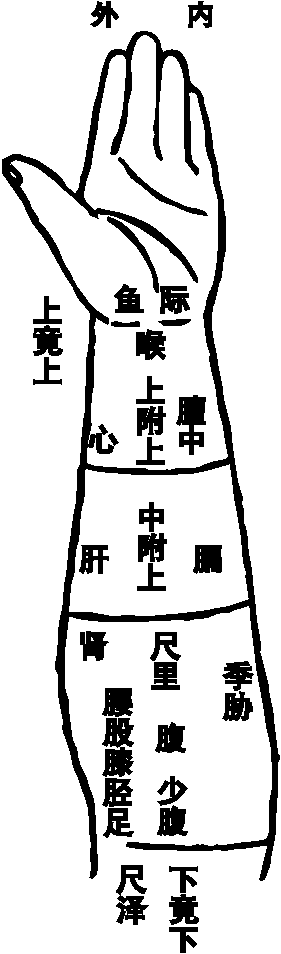
\includegraphics[width=0.14\textwidth]{尺肤切诊部位示意图(左手).pdf}}
	\hspace{3mm}
	\subcaptionbox{右手}
		{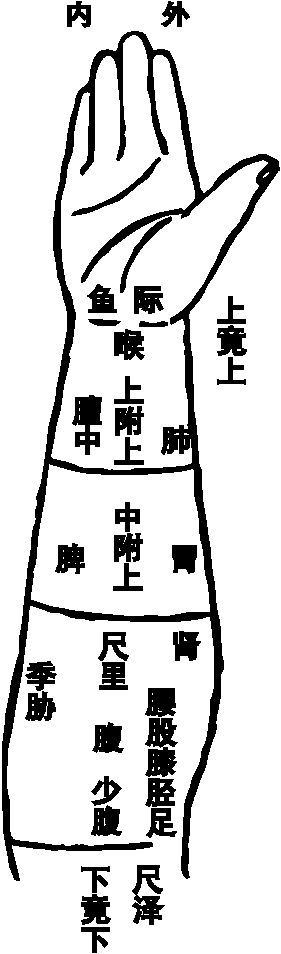
\includegraphics[width=0.14\textwidth]{尺肤切诊部位示意图(右手).pdf}}
	\caption{尺肤切诊部位示意图}
	\label{fig:尺肤切诊部位示意图} %% label for entire figure
\end{wrapfigure}
对“尺内两旁,则季胁也,……少腹腰股膝胫足中事也。”段的注释、理解,有三种观点:一是杨上善、王冰等认为是诊尺肤的脏腑身躯分候部位。(可参图\ref{fig:尺肤切诊部位示意图},详其义。)二是马莳、张介宾等认为是论述以气口寸、关、尺三部脉来诊察脏腑身躯。马莳曰:“后世王叔和之脉,其分部与此大同也欤。”三是认为是指全身诊察法而言,如近人时逸人曰:“《内经》原意系全身诊察法,所谓尺内两旁则季肋也,臂肘湾为尺泽部位,身躯两旁当臂肘湾处,即为季肋。其余则以尺肘部为基础,说明诸脏器邻近之部位,词意非常明显,无庸怀疑。后人误会,硬将全身诊察方法分配于手腕寸关尺三部。”

丹波元简对尺诊之所指作了详细的考察,他在《素问识》中说:“王冰注:‘尺内,谓尺泽之内也。’此即诊尺肤之部位。《平人气象论》云:‘尺涩脉滑,尺寒脉细。’王注亦云‘谓尺肤也’。《邪气脏腑病形》篇云;‘善调尺者,不待于寸。’又云:‘夫色脉与尺之相应,如桴鼓影响之相应也。’《论疾诊尺》篇云‘尺肤泽’,又云‘尺肉弱’。《十三难》云:‘脉数尺之皮肤亦数,脉急尺之皮肤亦急。’《史记·仓公传》亦云:‘切其脉,循其尺。’仲景云‘按寸不及尺’。皆其义也……明是尺即谓臂内一尺之部分,而绝非寸关尺之尺也。寸口分寸关尺三部仿于《难经》,马、张诸家以寸关尺之尺释之,与经旨差矣。”丹波氏之说可从。不过,本段原文虽非论寸口分为寸关尺三部以诊各脏腑,但《难经》关于寸关尺之脏腑划分的观点,其学术渊源显然与本段经旨密切相关,而后世盛行的“左手心肝肾,右手肺脾命”的寸关尺脉象定位说,显然是在本段尺肤诊脏腑定位的启迪下形成的。

\biaoti{【临证指要】}

1.色脉互参的临证意义

色脉互参是四诊合参的重要内容,脉诊可直接诊其内在经脉气血变化,面色是脏腑气血的盛衰和病变反映于外较易诊察者,因此《内经》常用色脉互参的方法诊断疾病,并有诸多的举例,如本段“征其脉小色不夺者,新病也;……征其脉与五色俱不夺者,新病也。”就是色脉互参诊病的一典型范例,以色脉互参的方法,来了解疾病的新久吉凶。

《内经》对于难以把握的真脏脉,也是以色脉互参之法来判断。《素问·玉机真脏论》曰:“真肝脉至,中外急,如循刀刃,责责然,如按琴瑟弦,色青白不泽,毛折乃死。”说明确诊是否肝真脏脉,除了脉诊外还应结合望面部之色,若已有本脏之肝木青色,还见所不胜之肺金白色,及全身衰败的表现,据此可确诊为肝的真脏脉,并可判断其预后凶险。

《难经》对色脉互参亦十分重视,如《难经·十三难》曰:“经言见其色而不得其脉,反得相胜之脉者即死;得相生之脉者病即自已。”,在四诊中,问诊从病人或他人处而得,闻诊主要是闻声、闻气味。在病人不发言语,又无他人提供病情的情况下,只有采取望诊与脉诊,要靠医生充分发挥主观能动性,尽心尽力而得,这也是《内经》屡论色脉互参的意义所在。

2.尺肤诊的临证意义

尺肤诊是《内经》所创立的特有诊病方法,在《内经》切诊中占有重要地位,其内容除散见诸篇外,尚有《灵枢·论疾诊尺》专篇论。诊尺肤主要是诊察尺肤部皮肉的大、小、缓、急、滑、涩及温度的变化,故《灵枢·论疾诊尺》曰:“审其尺之缓急小大滑涩,肉之坚脆而病形定矣。”从临床上来看,可有以下意义。①可判定病位:如本段所言“尺内两旁,则季胁也,……少腹腰股膝胫足中事也。”②可判断病因病性:如《灵枢·论疾诊尺》曰:“尺肤滑,其淖泽者,风也;尺肉弱者,解㑊、安卧;脱肉者,寒热不治;尺肤滑而泽脂者,风也;尺肤涩者,风痹也;尺肤粗如枯鱼之鳞者,水泆饮也。”③尺脉结合,全而认识疾病:·如《灵枢·论疾诊尺》曰:“尺肤热甚,脉盛躁者,病温也,其脉盛而滑者,病且出也。尺肤寒,其脉小者,泄,少气。”“尺炬然热,人迎大者,当夺血。尺坚大,脉小甚,少气,悗有加,立死。”《素问·平人气象论》也有尺脉合参的记载。后世医家对尺肤诊在临床上应用较少,作为切诊方法之一,有待进一步研究。

\section{素問·平人氣象論(節選)}%第二节

\biaoti{【原文】}

\begin{yuanwen}
黃帝問曰:平人何如?岐伯對曰:人一呼脈再動,一吸脈亦再動,呼吸定息\sb{1},脈五動,閏以太息\sb{2},命曰平人。平人者,不病也。常以不病調病人\sb{3},醫不病,故為病人平息以調之為法\sb{4}。

人一呼脈一動,一吸脈一動,曰少氣\sb{5}。人一呼脈三動,一吸脈三動而躁,尺熱曰病温,尺不熱脈滑曰病風,脈濇曰痹\sb{6}。人一呼脈四動以上曰死,脈绝不至曰死,乍踈乍數曰死\sb{7}。
\end{yuanwen}

\biaoti{【校注】}

\begin{jiaozhu}
	\item 呼吸定息:张介宾注:“呼吸定息,谓一息既尽,而换息未起之际也。”
	\item 闰以太息:闰,余也。张志聪注:“太息者,呼吸定息之时,有余不尽而脉又一动,如岁余之有闰也。”
	\item 常以不病调病人:不病,无病健康的人;调(diào),算度、计算、衡量。意为要以健康人(医生)的呼吸来衡量病人的脉息。
	\item 平息以调之为法:平息,即均匀呼吸。调之,衡量病人的脉息至数。吴昆注:“医不病则呼吸调匀,故能为病人平息以调脉。若医者病寒则呼吸迟,病人脉类于数。医者病热则呼吸疾,病人之脉类于迟,皆不足以调病人之脉也。”
	\item 少气:张介宾注:“脉为血气之道路,而脉之运行在乎气,若一呼一吸脉各一动,则一息二至,减少常人之半矣,以正气衰竭也,故曰少气。”
	\item 人一呼脉三动,……脉涩曰痹:尺,指尺肤。濇,同涩。张介宾注:“若不因定息太息而呼吸各三动,是一息六至矣,《难经》谓之离经。躁者,急疾之谓。尺热,言尺中近臂之处有热者,必其通身皆热也。脉数躁而身有热,故知为病温。数滑而尺不热者,阳邪盛也,故当病风;然风之伤人,其变不一,不独在于肌表,故尺不热也。濇为血不调,故当病痹”。
	\item 人一呼脉四动以上曰死,……乍疏乍数曰死:高世栻注:“人一呼脉四动以上,则太过之极。脉绝不至,则不及之极,乍疏乍数,则错乱之极。故皆曰死。”
\end{jiaozhu}

\biaoti{【临证指要】}

\xiaobt{“平息以调之为法”的临证意义}

本段主要论述以脉律来判断平脉、病脉、死脉的诊脉方法,是诊脉的基本要求,一直为后世遵循,沿用至今。

脉理精深微妙,不易掌握,脉象不仅有不易体察的四时权衡规矩沉浮之纲,又有历代二十四、二十八、三十等各家之说,正如陈念祖《医学实在易·八纲脉论》曰:“脉之为道,最为微渺而难知也。方书论脉愈详,而指下愈乱。”故前贤为使习医者切脉辨病能入门执要,提出了当先习知脉之大纲,有谓脉有四纲者,或曰浮、沉、迟、数,或曰迟、数、大、小。有谓脉有六纲者,如周学海《脉简补义·切脉大旨》曰:“《灵枢·邪气脏腑病形》以缓、急、大、小、滑、涩立纲,而以微甚纬之,实开千古诊法之奥,后世有以浮、沉、迟、数分纲者,则其义浅而不备矣。”有谓脉有八纲者,如陈念祖《医学实在易·八纲脉论》指出为浮、沉、迟、数、细、大、短、长。

综观各家之论,不论几脉为纲,其迟、数均为其要,《难经·九难》更认为“数者腑也,迟者脏也。数则为热,迟则为寒。诸阳为热,诸阴为寒,故以别知脏腑之病也。”迟数不仅是辨脏腑寒热阴阳之纲,同时也是易于掌握的,故本篇先论其辨识之法。

\biaoti{【原文】}

\begin{yuanwen}
平人之常氣禀於胃;胃者,平人之常氣也\sb{1}。人無胃氣曰逆,逆者死。春胃微弦曰平\sb{2},弦多胃少曰肝病,但弦無胃曰死\sb{3}。胃而有毛曰秋病,毛甚曰今病\sb{4},藏真散於肝,肝藏筋膜之氣也\sb{5},夏胃微鈎\sb{6}曰平,鈎多胃少曰心病,但钩無胃曰死;胃而有石曰冬病,石甚曰今病,藏真通于心,心藏血脈之氣也。長夏胃微耎弱\sb{7}曰平,弱多胃少曰脾病,但代\sb{8}無胃曰死;耎弱有石曰冬病,弱甚曰今病\sb{9}。藏真濡於脾,脾藏肌肉之氣也。秋胃微毛\sb{10}曰平,毛多胃少曰肺病,但毛無胃曰死;毛而有弦曰春病,弦甚曰今病,藏真高於肺,以行榮衛陰陽也。冬胃微石\sb{11}曰平,石多胃少曰腎病,但石無胃曰死;石而有鈎曰夏病,鈎甚曰今病,藏真下於腎,腎藏骨髓之气也。
\end{yuanwen}

\biaoti{【校注】}

\begin{jiaozhu}
	\item 胃者,平人之常气也:常气,正常人的脉气。意为无病正常人脉象应具有胃气。
	\item 春胃微弦曰平:春季(肝脏)脉有胃气而略带弦,是正常的脉。吴昆注:“弦,脉引而长,若琴弦也。胃,冲和之名。春脉宜弦,必于冲和之中微带弦,是曰平调之脉。”下文“夏胃微钩”、“长夏胃微耎弱”等,义皆同此。
	\item 弦多胃少曰肝病,但弦无胃曰死;吴昆注:“弦多胃少,是肝木偏胜而失其冲和之气,故为肝病。但弦急之脉,更无冲和之气,是失其生道。故死。”下文“钩多胃少”、“弱多胃少”、“但钩无胃”、“但石无胃”等,义皆同此。
	\item 胃而有毛曰秋病,毛甚曰今病:张介宾注:“毛为秋脉属金,春时得之,是谓贼邪,以胃气尚存,故至秋而后病。春脉毛甚,则木被金伤,故不必至秋,今即病矣。”
	\item 脏真散于肝,肝藏筋膜之气:脏真,指五脏所藏的真气。吴昆注:“春时肝木用事,故五脏天真之气,皆散于肝。”肝主筋,故肝藏筋膜之气。下文“通于心”、“濡于脾”、“高于肺”、“下于肾”义皆仿此。高世栻注:“盖肝主疏泄,故曰散。心主血脉,故曰通。脾主灌溉,故曰濡。肺位居上,故曰高。肾为水脏,故曰下也。”
	\item 钩:夏季主脉,即洪大脉,如钩端微曲之象。
	\item 耎弱:耎,同软。耎弱,指柔和而不劲急的脉象,为脾脏主脉。
	\item 代:其义有两说,一是谓弱极,如高世栻注:“代,软弱之极也。软弱极而无胃气,则曰死脉。”一是谓更代,如张介宾注:“代,更代也。脾主四季,脉当随时而更,然必欲皆兼和耎,方得脾脉之平。若四季相代,而但弦、但钩、但毛、但石,是但代无胃,现真脏也,故曰死。”
	\item 耎弱有石曰冬病,弱甚曰今病:弱甚,《甲乙经·卷四》、《千金要方·卷十五》均作“石甚”。张介宾注:“石为冬脉属水,长夏阳气正盛而见沉石之脉,以火土气衰,而水反乘也,故至冬而病。弱,当作石。长夏石甚者,火土大衰,故不必至冬,今即病矣。”
	\item 毛:秋季主脉,似浮脉。王冰注:“谓如物之浮,如风吹毛也。”
	\item 石:冬季主脉,脉来沉而实,如石沉水中。
\end{jiaozhu}

\biaoti{【理论阐释】}

\xiaobt{脉以胃气为本}

辨五脏之脉的平脉、病脉、死脉以及兼脉,主要是据脉中的“胃气”。所谓“胃气”不仅指胃本身具有的受纳、腐熟、和降等功能,而且还包含胃腑机能在整个机体中的作用,故“胃气”与人的生命息息相关,正如本篇说:“人以水谷为本,故人绝水谷则死,脉无胃气亦死。”又说:“平人之常气禀于胃,胃者,平人之常气也,人无胃气曰逆,逆者死。”

脉以胃气为本,其理如下:①脉气根源于五脏六腑,胃为之本。《素问·调经论》曰:“五脏之道,皆出于经隧,以行血气。”五脏功能活动依赖于胃气,正如《素问·玉机真脏论》所说:“五脏者,皆禀气于胃,胃者五脏之本也。”②脉中血气源于水谷之气。《灵枢·本脏》曰:“经脉者,所以行血气而营阴阳……是故血和则经脉流行。”人生理活动所需要的各种精气均由水谷之气所化,如《灵枢·决气》论述了六气(精、气、血、津、液、脉)由一气(水谷之气)而化,最后又强调曰:“六气者然五谷与胃为大海。”③肺气附于胃气,推动脉气运行。“诸气者皆属于肺”,脉气亦离不开肺气之助,然肺气能行血脉之中,常依附于胃化生的水谷之气,如《灵枢·动输》曰:“胃为五脏六腑之海,其清气上注于肺,肺气从太阴而行之。其行也以息往来,故人一呼脉再动,一吸脉亦再动,呼吸不已,故动而不止。”④胃气运脏真之气于脉中。脏真之气是五脏之先天真气,然其必依赖胃气才能行于经脉之中,在全身发挥其应有的功能,所以《素问·玉机真脏论》说:“脏气者,不能自致于手太阴,必因于胃气,乃至于手太阴也。”

由于经脉的正常活动依赖胃气,所以五脏应时之气与饱满的胃气相合,表现于脉中,才是五脏康健之正常脉象,若胃气不足则为五脏病脉,只有应时之脉而无胃气,则为毫无生机的五脏死脉,又称真脏脉。

\biaoti{【临证指要】}

\xiaobt{脉以胃气为本的临床意义}

《内经》脉以胃气为本的观点,对后世脉学的发展具有十分重要的影响,并且为后世临床重视胃气,尤其对治疗重病危症更需顾护胃气,以及脾为后天之本理论的提出,均具有指导意义。

何谓脉有胃气,《素问·玉机真脏论》曰:“脉弱以滑,是有胃气。”此处之“弱”是柔和之意,滑指脉来流利。《灵枢·终始》曰:“谷气来也徐而和。”此处的“谷气”即指脉之胃气。故张介宾曰:“自有一种雍容和缓之状者,便是有胃气之脉。”因此可以说,凡脉来和缓均匀、不浮不沉、不大不小、不疾不徐、不长不短,应手柔和有力、来去节律整齐,有生机勃勃之象的脉,便是有胃气之脉。历代医家对胃脉的形态以及临床应用多有阐发,使诊察脉象有无胃气成为临床预后疾病的重要内容。如张介宾《景岳全书·胃气解》曰:“察之之法,如今日尚和缓,明日更弦急,知邪气之愈进,邪愈进则病愈甚矣;今日甚弦急,明日稍和缓,知胃气之渐至,胃气至则病渐轻矣。即如顷刻之间,初急后缓者,胃气之来也;初缓后急者,胃气之去也,此察邪正进退之法也。至于生死之兆,亦唯以胃气为主。”当今中医认为平人之脉不但要有“胃气”,而且还要具备“有神”、“有根”的特点。实际上脉的神、根仍然是在“脉以胃气为本”的基础上发展起来的。

“以胃气为本”的理论还应用到其他诊法之中,如胃气是舌苔形成的基础,故望舌苔以判断胃气的盛衰、邪气的进退。在问诊方面,若粥架不入,知其胃气衰败,预后不良等。

\biaoti{【原文】}

\begin{yuanwen}
胃之大絡,名曰虚里\sb{1},贯鬲絡肺,出於左乳下,其動應衣,脈宗氣也\sb{2}。盛喘數絕者,則病在中\sb{2};結而横,有積矣\sb{4};絕不至,日死。乳之下,其動應衣,宗气泄也\sb{5}。
\end{yuanwen}

\biaoti{【校注】}

\begin{jiaozhu}
	\item 虚里:是足阳明胃经除丰隆外的又一大的络脉,其脉从胃贯穿膈膜络于肺,出于左乳下。后世亦将心尖搏动处,谓之虚里。
	\item 其动应衣,脉宗气也:衣,《甲乙经》作“手”。脉,动词,诊察的意思。一说,“脉宗气”,作“脉气之宗解”。可参。
	\item 盛喘数绝者,则病在中:盛喘,指虚里处搏动之甚如气急之喘促;数,屡次之意;绝,断绝,指搏动停止。张介宾注:“若虚里动甚而如喘,或数急而兼断绝者,由中气不守而言,故曰病在中。”
	\item 结而横,有积矣:结,脉来迟,时一止;横,有充满、坚硬之意;积,指积聚之证。
	\item 乳之下,其动应衣,宗气泄也:吴昆注:“宗气宜藏不宜泄,乳下虚里之脉,其动应衣,是宗气失藏而外泄也。”
\end{jiaozhu}

\biaoti{【临证指要】}

\xiaobt{虚里诊法的临床价值}

经文举例说明了虚里诊四种情况:①虚里搏动“盛喘数绝”,反映体中的胃及心肺有疾;②虚里搏动“结而横”说明内有积聚;③若虚里搏动“绝不至”(跳动中断,绝而不复),预后不良;④搏动剧烈,“其动应衣”,是宗气大泄之证,预后亦差。经文虽然简短,但颇被后世医家重视,如魏柳洲曰:“凡治小儿,不论诸证,宜先揣虚里穴,若跳甚者,不可攻伐,以其先天不足故也。”王士雄曰:“小儿则脉候难凭,揣此尤为可据。”此外,临证如遇暴厥、大虚大实脉伏不见之证,亦可应用虚里诊法,协助诊断。尽管这一古老的诊断方法在目前中医诊断学上很少提及,但其在临床上的价值是不能忽视的。

\biaoti{【原文】}

\begin{yuanwen}
頸脈動喘疾欬\sb{1},曰水。目裹微腫,如卧蠶起之狀\sb{2},曰水。溺黄赤安卧者,黄疸\sb{3}。已食如飢者,胃疸\sb{4}。面腫曰風,足脛腫曰水。目黄者曰黄疸。婦人手少陰脈\sb{5}動甚者,妊子也。

脈有逆從四時,未有藏形\sb{6},春夏而脈瘦\sb{7},秋冬而脈浮大,命曰逆四時也。風熱而脈靜,泄而脱血脈實,病在中脈虚,病在外脈濇堅者,皆難治,命曰反四時也\sb{8}。
\end{yuanwen}

\biaoti{【校注】}

\begin{jiaozhu}
	\item 颈脉动喘疾咳:颈脉,即人迎脉,属足阳明胃经。张介宾注:“水气上逆,反侵阳明则颈脉动。水溢于肺,则喘急而疾咳。”
	\item 目裹微肿,如卧蚕起之状:张介宾注:“目裹者,目下之胞也,胃脉之所至,脾气之所主,若见微肿如卧蚕起之状,是水气淫及脾胃也。”
	\item 黄疸:病证名,多由湿热或寒湿内阻中焦所致。
	\item 胃疸:疸,与瘅通,热也。王冰注:“是则冒热也,热则消谷,故食己如饥也。”
	\item 手少阴脉;指神门穴部位之脉。王冰注:“手少阴脉,谓掌后陷者中,当小指动而应手者也。”
	\item 未有脏形:脏形,即五脏应四时的正常脉象。未有脏形,是指不见本脏应时的脉象。
	\item 脉瘦:指沉细脉象。
	\item 风热而脉静,……命曰反四时也:马莳注:“此言脉与病反者,是亦脉与时反之意也。病由风热,脉宜浮大而反沉静,则阳病见阴脉也。泄利脱血二证,脉宜沉细而反实大,则阴病见阳脉也。病在中者,脉为有力,则中气方盛,今脉反虚;病在外者,脉宜浮虚,则表病易痊,今脉反涩坚,是皆难治之证,犹脉之反四时也。”
\end{jiaozhu}

\biaoti{【理论阐释】}

\xiaobt{妊娠脉的诊断}

本段提到了妊娠脉的诊断“妇人手少阴脉动甚者,妊子也。”与《灵枢·论疾诊尺》中“女子手少阴脉动甚者妊子”同,手少阴究竟何指,历代注家意见不一。①王冰谓手少阴神门穴处的搏动。②张志聪、高世栻认为是两手寸口脉的尺部,如高氏曰:“少阴,尺脉也……两手少阴脉动甚者,则知肾气有余,感天一所生之气,故妊子也。”③马莳认为是左手寸口的寸部。注曰:“左手寸部属手少阴心经……故知手少阴之脉动甚者,为妊男子也。”④认为“手少阴”当作“足少阴”。如《新校正》云:“按全元起本作足少阴。”

验之临床,高氏、张氏意见可从,这与《素问·阴阳别论》所说的“阴搏阳别,谓之有子”的精神一致。关前为阳以候心,关后为阴以候肾。一般认为尺部脉象滑利有力是妊娠的脉候。但按神门穴在临床上也有应用。如张志聪“左手少阴肾脉动甚者,当妊子,以左男而右女”的说法,亦为目前少数医者所认同。

总之,以脉辨妊娠在临床上有其一定价值。因为妊娠期间机体有效循环血量显著增加,超过正常血液总量的33\%以上,此时心脏的收缩力量显著加强,每次搏出量增加,因而脉搏就相应地有力流畅,尽管脉象的形成受多种因素影响,但有效循环血量和心脏收缩力毕竟起着重要的作用,可见,古人凭脉辨妊娠的方法有其一定生理基础。当然在运用这一诊脉方法时,还需结合其月经史以及有关情况,才能做出准确的判断。

\section{靈樞·五色(節選)}%第三節

\biaoti{【原文】}

\begin{yuanwen}
雷公曰:五官之辨奈何?黃帝曰:明堂骨高以起,平以直\sb{1},五藏次於中央,六府挾其兩側\sb{2},首面上於闕庭\sb{3},王宫在於下極\sb{4},五藏安於胸中\sb{5},真色以致\sb{6},病色不見,明堂潤澤以清\sb{7},五官惡\sb{8}得無辨乎……

沉濁為內,浮澤為外\sb{9},黃赤為風,青黑為痛,白為寒\sb{10},黃而膏潤為膿,赤甚者為血\sb{11},痛甚為攣,寒甚為皮不仁\sb{12}。五色各見其部,察其浮沉,以知淺深\sb{13};察其澤夭,以觀成敗\sb{14};察其散搏,以知遠近\sb{15};視色上下,以知病處\sb{16};積神於心,以知往今\sb{17}。
\end{yuanwen}

\biaoti{【校注】}

\begin{jiaozhu}
	\item 明堂骨高以起,平以直:明堂,本指古时帝王宣明政教之处,此指鼻部。意为鼻骨高隆起,平正而端直。
	\item 五脏次于中央,六腑挟其两侧:五脏所主部位依此排列在面部的中央,六腑所主部位则挟于其两旁。
	\item 首面上于阙庭;阏,宫门外两侧的楼台,中间有道路,其处置门,谓之阙门,本篇以阙门比喻两眉间:庭,堂阶前的地坪,本篇以庭比喻前额部。意为头面部各组织器官的情况向上反映于两眉之间和前额。
	\item 王宫在于下极:王宫,帝王的宫室,此指心脏;下极,即两目之间。意为心脏的情况反映于两目之间的部位。
	\item 胸中:胸腹之中。
	\item 真色以致:真色,正色,为脏腑和调,精气充盈的表现;致,到达、表达。意为正色显现于面部。
	\item 清:清纯、洁净,不污浊。
	\item 恶:怎么,表示反对。
	\item 沉浊为内,浮泽为外:面色沉滞晦浊的为病在里,浮润光泽的为病在表。
	\item 黄赤为风,青黑为痛,白为寒:面色见黄赤的多属逢热一类疾病;青黑色多为血气凝滞,故属疼痛一类的疾病;白色多为寒病。
	\item 黄而膏润为脓,赤甚者为血:此指疮疡而言。
	\item 痛甚为挛,寒甚为皮不仁:不仁,皮肉不知痛痒,感觉迟钝。面色青黑主痛证,而青黑过重主拘挛;面色白主寒证,白色太重主皮肤不仁。
	\item 察其浮沉,以知浅深:色浮者主病浅,色沉者主病深。
	\item 察其夭泽,以观成败:据面色的夭枯与润泽判断预后。
	\item 察其散抟,以知远近:抟,凝聚。病色散而不聚的为病程短暂;病色聚面不散的为病久远。
	\item 视色上下,以知病处:察病色在面部上下脏腑肢节所应的部位,则可了解疾病所在之处。
	\item 积神于心,以知往今:医生察面色时应聚精会神、专心致志,这样才可了解疾病的发展变化。
\end{jiaozhu}

\biaoti{【理论阐解】}

\xiaobt{望面色诊病之理}

人有五脏现五色,以面部表现最为明显,故望面色是望诊的重要内容,面望面色主要是观察病人面部的色泽及异常之色所出现的部位。

本篇以整体观为指导,详细地叙述了五脏六腑,四肢关节在面部相应的望色部位,指出“五脏次于中央,六腑挟共两侧”,“五色之见也各出其色部”。《灵枢·邪气脏腑病形》也曰:“十二经脉,三百六十五络,其血气皆上于面”。正是由于经脉气血的联系,面部可为全身脏腑肢节的缩影,故可以反映脏腑肢节的病理变化。

这种以局部为整体一个缩影的论述,与现代生物全息思想有相通之处。根据生物全息律的一般原理,人体的任何一相对独立的部位,如每一肢节,每一器官,也应寓藏着整个机体的生命信息。从信息角度而言,也可以说经络是一人体信息的通道,气血是信息的载体,十二经脉之气血皆上于面,将整体的信息传输于面部,使面部成为全身的缩影,因而通过面部不同部位的色泽变化可以诊断全身疾病。

\biaoti{【临证指要】}

\xiaobt{察面色的临床运用}

临床上诊察面色测知疾病,有以下几个方面。①察色要做到全神贯注,细心观察,诊断才能正确。②从面部病色出现与脏腑肢节相应的部位,诊知疾病所在。③察色浮沉,可辨病位的表里深浅。④察五色不同,可辨病因,定病性,即“黄赤为风,青黑为痛,白为寒。”⑤可判定一些病症,如“黄而膏润为脓,赤甚者为血”,“病甚为挛,寒甚为皮不仁。”⑥察色散抟,辨别病程长短“远近”。⑦察色清浊,测知病情的轻重。⑧察色夭泽,辨病吉凶,这些与《素问·脉要精微论》所论五欲、五不欲的精神是一致的。

后世医家在运用《内经》理论基础上又各从不同方面有所发展。如清·汪宏《望诊遵经》提出望浮沉、清浊、微甚、散抟,泽夭十法,用以鉴别疾病的表里、阴阳、虚实、新久、轻重。若将面色各部综合运用,更能辨病入微。如眼黑为痰饮中停,颧红为火热内盛,故眼黑颧红则主痰热等。

\xiaojie

本章所选经文篇章虽不多,但已涉及到诊法诸方面的内容。

1.对诊法的要求,提出了“虚静为保”、“诊法常以平旦”等,其精神实质为诊病是一个十分慎重的事情,要环境相对安静、病人心情安稳,医生更应专心致志。这不仅是准确获得病情的基础,也反映出医德医风之渊源。

2.应多诊合参,对望诊、切诊合参论述较多,如色脉合参,寸尺合参等。后世遵其理,提出了四诊合参,以求病本,使中医诊断更具特色。

3.切诊尤其脉诊是本章的主要内容:①脉诊可以诊断全身的气血盛衰。诊脉的方法,是“常以不病调病人”、“平息以调之为法”。②论述了脉应四时,提示诊脉要注意天人相应的关系。③脉以胃气为本,据胃气的有无多少判断平脉、病脉、死脉,无胃气的脉,就是死脉,又称真脏脉。这种重视胃气的思想,不仅对后世的脉学有着深刻的影响,而且对中医理论的发展以及临床治疗等方面都有十分重要的指导意义。④尺肤和虚里的诊断方法及诊断意义。⑤脉有逆从阴阳的论述,对疾病的预后有着重要意义,亦说明了疾病的复杂性,临床需辨真伪,由此后世提出了舍脉从证,舍证从脉等权变之法。

4.关于望诊,本章论述了望眼神、望面色以及望形态。对望面色的意义、临床应用进行了说明,对望面色的要点阐述详明。为望诊的发展奠定了基础。

5.对问诊、闻诊本章也有一定的论述,如“声如从室中言”、“水泉不止”、释梦诊病等,皆是闻诊和问诊的内容。

\zuozhe{(周发祥)}
\ifx \allfiles \undefined
\end{document}
\fi